%
% Master thesis template for Ghent University (2018)
%
%
%  !!!!!!!!!!!!!!!!!!!!!!!!!!!!!!!!!!!!!!!!!!!!!!!!!!!!!!!!!!!!
%  !!  MAKE SURE TO SET lualatex OR xelatex AS LATEX ENGINE  !!
%  !!!!!!!!!!!!!!!!!!!!!!!!!!!!!!!!!!!!!!!!!!!!!!!!!!!!!!!!!!!!
%  !! For overleaf:                                          !!
%  !!     1. click gear icon in top right                    !!
%  !!     2. select `lualatex` in "latex engine"             !!
%  !!     3. click "save project settings"                   !!
%  !!                                                        !!
%  !!!!!!!!!!!!!!!!!!!!!!!!!!!!!!!!!!!!!!!!!!!!!!!!!!!!!!!!!!!!
%
%
%  History
%    2014         Doctoral Thesis of Bruno Volckaert
%    2017         Adapted to master thesis by Jerico Moeyersons
%    2018         Cleanup by Merlijn Sebrechts
%
%  Latest version
%    https://github.com/galgalesh/masterproef-template
%
\documentclass[11pt,a4paper,twoside, openany]{book}
\usepackage[a4paper,includeheadfoot,margin=2.50cm]{geometry}

\setlength{\parindent}{0cm}           % indent of the first sentence of a paragraph
\setlength{\parskip}{1em}             % space between paragraphs
\renewcommand{\baselinestretch}{1.2}  % stretch horizontal space between everything

\usepackage{graphicx}
\graphicspath{{images/}}
\usepackage{pdfpages}
\usepackage{enumitem}
\usepackage{mathtools}
\usepackage{float}
\usepackage{caption}
\usepackage{subcaption}
\usepackage[toc,page]{appendix}
\usepackage{minted}                                    % for modern code highlighting
\newenvironment{code}{\captionsetup{type=listing}}{}   % To get multiline code fragments working: https://tex.stackexchange.com/a/53540/72273

\usepackage{upquote}


\PassOptionsToPackage{hyphens}{url}
\usepackage{hyperref}
\usepackage{url}

\usepackage{quotchap}              % For the fancy quotes next to the chapter titles

%\usepackage[numbers]{natbib}       % For bibliography; use numeric citations
%\bibliographystyle{IEEEtran}
%\usepackage[nottoc]{tocbibind}     % Put Bibliography in ToC

%
% pseudocode
%
\usepackage{amsmath}
\usepackage{algorithm}
\usepackage[noend]{algpseudocode}

%
% Charts and plots
%
\usepackage{pgfplots}
%
% Glossaries
%
\usepackage[acronym,toc]{glossaries}
\makeglossaries

%
% Defines \checkmark to draw a checkmark
%
\usepackage{tikz}
\def\checkmark{\tikz\fill[scale=0.4](0,.35) -- (.25,0) -- (1,.7) -- (.25,.15) -- cycle;}

%
% For tables
%
\usepackage{booktabs}
\usepackage{array}
\usepackage{ragged2e}  % for '\RaggedRight' macro (allows hyphenation)
\newcolumntype{L}[1]{>{\raggedright\let\newline\\\arraybackslash\hspace{0pt}}m{#1}}
\newcolumntype{C}[1]{>{\centering\let\newline\\\arraybackslash\hspace{0pt}}m{#1}}
\newcolumntype{R}[1]{>{\raggedleft\let\newline\\\arraybackslash\hspace{0pt}}m{#1}}

%
% Set the title and your name
%
\title{Evaluating the human exposure of a UAV-aided network}
\author{Thomas Detemmerman}

%
%  END OF HEADER
%  The actual latex document content starts here.
%
\begin{document}

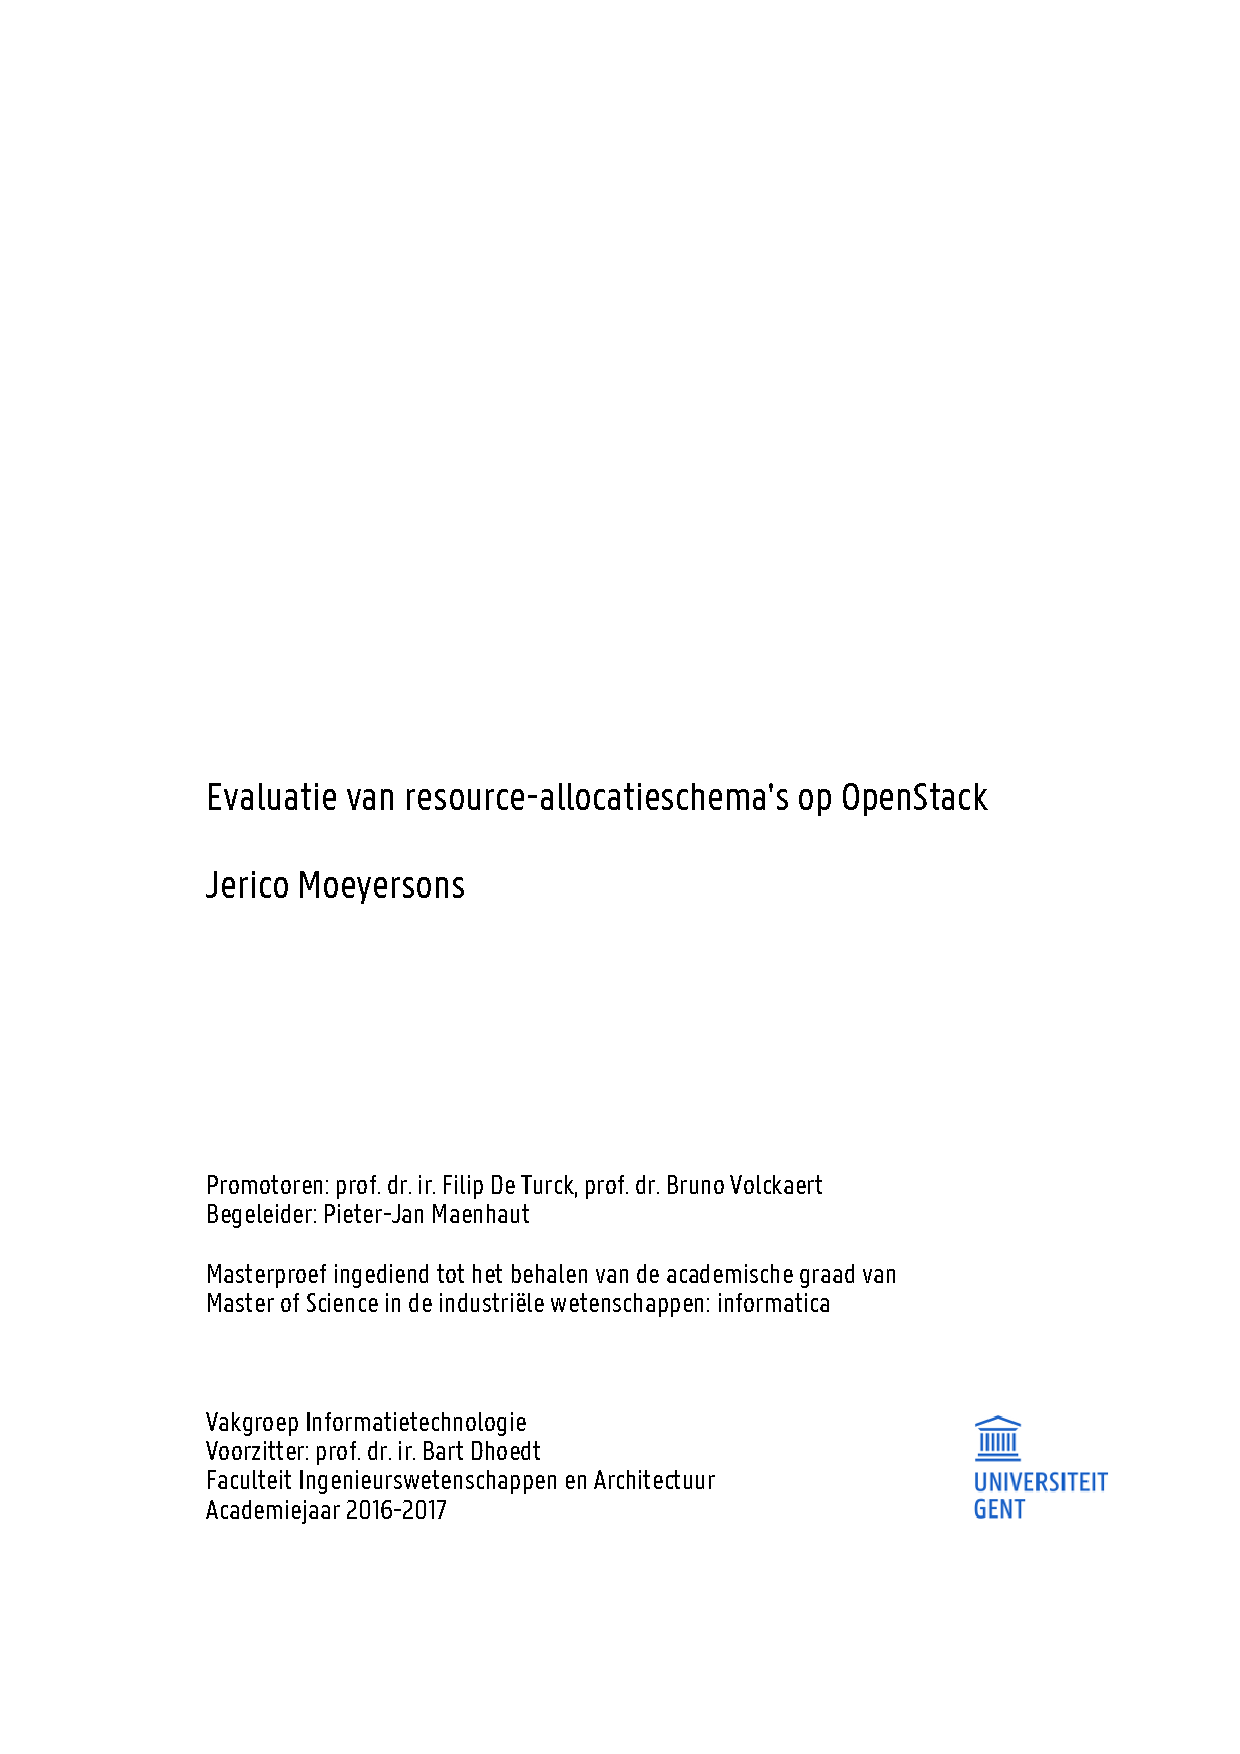
\includepdf{voorblad.pdf}             % Front matter
\newpage\thispagestyle{empty}\mbox{}  % White page
\thispagestyle{empty}    % Don't show page number

\begin{center}
\textbf{Dankwoord}
\end{center}

Na een intensieve periode van vijf maanden heb ik de laatste hand gelegd aan deze masterproef. Op verschillende vlakken heb ik nieuwe elementen binnen de wondere wereld van de informatica kunnen ontdekken. Daarom wil ik aan een aantal personen een welgemeende dankjewel zeggen om mij steeds te steunen tijdens het maken van deze masterproef.\\

Allereerst wil ik mijn promotoren, prof. dr. ir. Filip De Turck en prof. dr. Bruno Volckaert, bedanken voor het vertrouwen, de steun, de tips en de feedback. Ook mijn begeleider, de heer Pieter-Jan Maenhaut wil ik hartelijk bedanken voor de steun, de vele tips en uitgebreide feedback. Daarnaast wil ik ook mevrouw Leen Pollefliet bedanken voor de vele tips die ik nuttig heb kunnen gebruiken tijdens het schrijven en presenteren van deze masterproef. Vervolgens wil ik ook mijn vriendin, Lynn Haentjens, hartelijk bedanken om mij steeds te steunen in deze periode alsook voor het leveren van grammaticale feedback. Ten slotte wil ik ook mijn ouders bedanken voor de geleverde steun tijdens deze periode.\\

Om te eindigen met mijn dankwoord wil ik ook nog een aantal vrienden, namelijk Cédric Reyniers, Maxim Ronsse en Simon Vermeersch, bedanken voor de aangename middagpauzes, de relevante en ook de minder relevante gesprekken.\\
\\
Bedankt allemaal!\\
Jerico Moeyersons          % Word of thanks
%\newpage\thispagestyle{empty}\mbox{}  % White page
%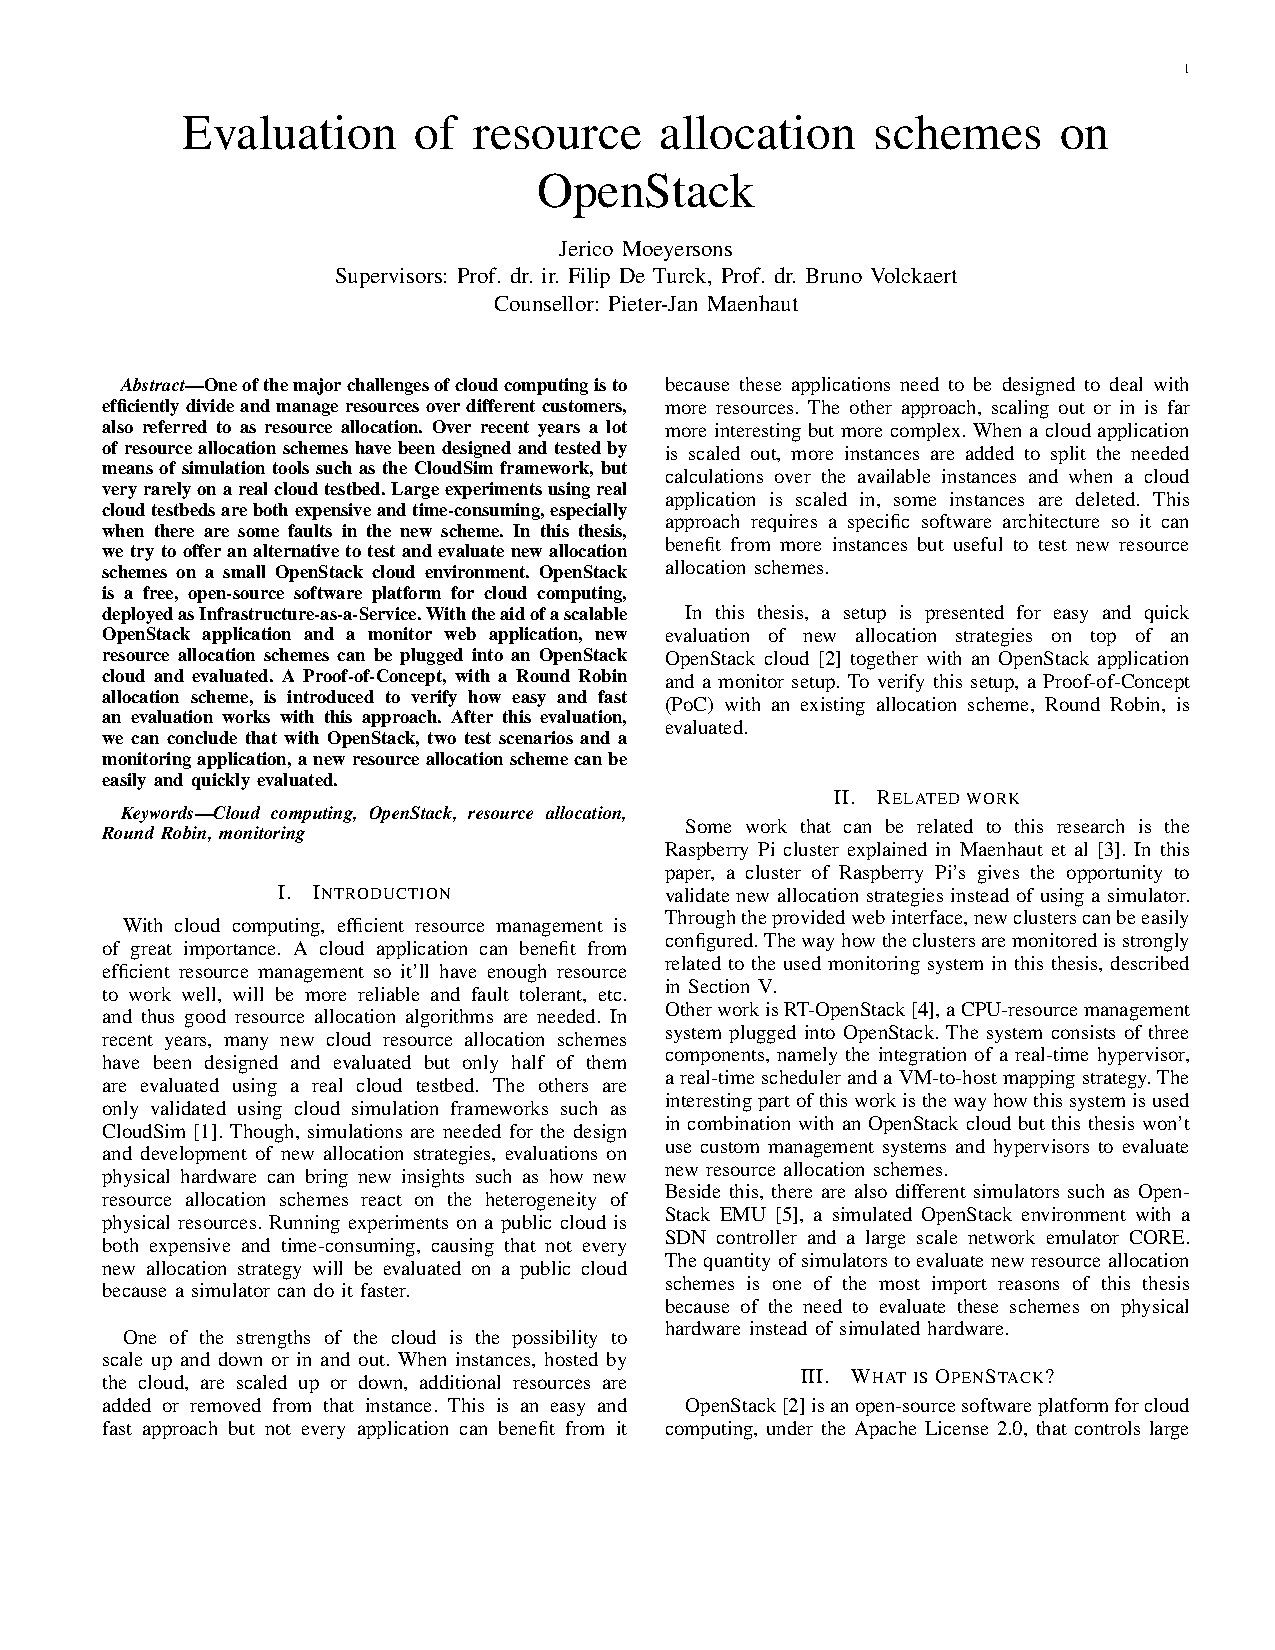
\includepdf[pages={-}]{abstract.pdf}  % Extended Abstract
\tableofcontents                      % Table of Contents
%\listoffigures                        % List of figures
%\listoftables                         % List of tables
%\listoflistings                       % List of listings (code fragments)



%-------------------------------- acroniemen

\newacronym{UABS}{UABS}{Unmanned Arial Base Station}
\newacronym{EIRP}{EIRP}{equivalent isotropic radiation power}
\newacronym{UE}{UE}{User Equipment}
\newacronym{IEC}{IEC}{International Electrotechnical Commission}
\newacronym{SAR}{SAR}{Specific Absorption Rate}
\newacronym{whipp}{WHIPP}{WiCa Heuristic Indoor Propagation Prediction}
\newacronym{DL}{DL}{downlink}
\newacronym{UL}{UL}{uplink}
\newacronym{LTE}{LTE}{Long-Term Evolution}
\newacronym{FDD}{FDD}{Frequency Division Duplex}
\newacronym{TDD}{TDD}{Time Division Duplex}
\newacronym{ICNIRP}{ICNIRP}{International Commission on Non-Ionizing Radiation Protection}
\newacronym{LOS}{LOS}{line of sight}
\newacronym{NLOS}{NLOS}{non line of sight}
\newacronym{Exp Opt}{Exp. Opt.}{exposure optimized}
\newacronym{PwrC Opt}{PwrC. Opt.}{power consuption optimized}
\newacronym{WHO}{WHO}{World Health Organization}
\newacronym{FCC}{FCC}{Federal Communications Commission}
\newacronym{USA}{USA}{United States of America}
\newacronym{IOT}{IoT}{Internet of Things}
\newacronym{UAV}{UAV}{Unmanned Aerial Vehicle}
\newacronym{EU}{EU}{European Union}
%--------------------------------- woordenlijst
\newglossaryentry{isotropicradiator}{
	name = equivalent isotropic radiator,
	text = equivalent isotropic radiator,
	description = A theoretical source of electromagnetic waves which radiates the same intensity for all directions
}

\newglossaryentry{spuriousradiation}{
	name = spurious radiation,
	text = spurious radiation,
	description = According to the thefreedictionary.com: Any emission from a radio transmitter at frequencies outside its frequency band. Also known as spurious emission
}

\newglossaryentry{RRP}{
	name = RRP,
	text = RRP,
	description = RRP is an abreviation used in this paper to indicate an extension on EIRP and stands for Real Radiation Pattern. An RRP value indicates the power (in dBm) for a certain location unlike an EIRP where the power (in dBm) is independent of the location
}

\newglossaryentry{power flux density}{
	name = power flux density,
	text = power flux density,
	description = Magnitude of power ($W$) that travels through a curtain area ($m^2$)
}

\newglossaryentry{thermoregulatory capacity}{
	name = thermoregulatory capacity,
	text = thermoregulatory capacity,
	description = The capacity of an organism to regulate body temperture
}

%\printglossary[type=\acronymtype,title={Lijst van acroniemen}]
%\addcontentsline{toc}{chapter}{\textcolor{maincolor}{Lijst van acroniemen}}
%\printglossary
%\addcontentsline{toc}{chapter}{\textcolor{maincolor}{Verklarende woordenlijst}}





\printglossaries

%
% Include the main chapters of the thesis below
%
% Inspirerende caption 
%
%\begin{savequote}[0.55\linewidth]
%	``If you think you've seen this movie before, you are right. Cloud computing is based on the time-sharing model we leveraged years ago before we could afford our own computers. The idea is to share computing power among many companies and people, thereby reducing the cost of that computing power to those who leverage it. The value of time share and the core value of cloud computing are pretty much the same, only the resources these days are much better and more cost effective.''
%	\qauthor{\textasciitilde David Linthicum, author of Cloud Computing and SOA Convergence in Your Enterprise: A Step-by-Step Guide}
%\end{savequote}

\chapter{Introduction}
\label{chap:intro}

\section{Outline of the issue} %1p
\label{sec:issue}



% inspiratie kan je hier ook nog vinden:
% PREDICTION AND COMPARISON OF DOWNLINK ELECTRICFIELDAND UPLINK LOCALISED SARVALUES FOR REALISTIC INDOORWIRELESS PLANNING
Society is constantly getting more and more dependent on electronic communication. On any given moment in any given location, an electronic device
can request to connect to the bigger wireless network. Devices need more then ever to be connected, starting from small IOT sensors up to self-driving cars
which needs to be supported by the existing infrastructure. 

Once again it becomes clear why we're on the eve of a new generation of cellular communication named 5G. 
This new technology is capable of handling millions of connections every square meter %to do: klopt deze hoeveelheid want lijkt wel heel veel.
while satisfying only a few microseconds of a delay and providing connections up to 10Gbps \cite{5GFeatures}.

Also in exceptional and possibly life-threatening situations, we rely on the cellular network. For example during the terrorist attacks in Zaventem, a Belgian city.
Mobile network operators saw all telecommunications drastically increasing causing moments of contention. Some operators decided to temporarily exceed the exposure limits in
order to handle all connections. \cite{baseZaventem}

Electromagnetic exposure can however not be neglected. Research shows how exesive electromagnetic radiation can cause diverse biological side effects \cite{bioeffects}.
Because of public concern, the World Health Organization had launched a large, multidisciplinary research effort which eventually concluded that there was no sufficient evidence that confirmed 
that exposure to low level electromagnetic fields harmfull is \cite{WHO}. Nevertheless remains the public very concerned about potetial health risks.

\section{Objective}
\label{sec:objective}

In this master dissertation the electromagnetic exposure of  a user is investigated taking all prominent sources into account which include the user's own mobile device, basestations
and other users their \gls{UE}.

In order to determine the magnitude of exposure to which users in a certain area are exposed, various values need to be known. 
Not only the used technology but also the position of users and basestations need to be known. 
To make this research possible, an existing planning tool is used which gives insight in users and basestation distributions. Bitrates of idividual users, power useage of 
the different electronical devices and which basestations handels which users. The tool describes in other words a fully configured network.
In this way, all needed parameters will be known.

The electromagnetic exposure will then be analysed by applieing the tool in different scenarios. During the simulations
it is investigated how various input variables influence the network.

The calculation of electromagnic exposure originating from base stations is discussed in variously discussed in litterture. Papers who convert electromagnetic exposure
 into a single value is rather limited.
Not only how electromagnetic exposure behaves but also related values like power consumption or even coverage.



\textbf{research question 1:} How can a \gls{UABS} network be optimized to minimize global exposure and overal power consumption? What are the effects on the network?\\

\textbf{research question 2:} What are the advantages and disadvantages of a model as described in research question 1 compared the the already existing pahtloss oriented model.\\

\textbf{research question 3:} How does the \gls{UABS} fly height influence uplink and downlink exposure?


%todo: onderstaande tekst (in commentaar) is een letterlijke copy van J10-RDP. Het is hier gezet als referentie. Moet nog correct verwoorden:
%In this paper, prediction algorithms are created to
%simulate and visualise electric-field strengths due to
%downlink traffic and localised SARvalues due to uplink
%traffic. Downlink exposure are expressed in terms of
%whole-body exposure due to the electric-fields E originating
%from the base stations or APs, whereas uplink
%exposure are expressed in terms of localised SAR10g
%[SAR in 10 g of tissue(8)] values due to the mobile
%device’s transmitted signal. To

\section{Structure}
\label{sec:structure}

TODO: update this section

The following chapter \ref{chap:stateoftheart} exists of several succesive sections explaining how the electromagnetic exposure of a single human being is calculated. The first section \ref{sec:calculatingexposure}
explains how the exposure is calculated between a user and a single femtocell. Section \ref{sec:combiningexposure}  defines how to combine all exposures from the different femtocells towards a single users.
Finaly, section \ref{sec:radiationpatterns} explains how directional antenna's are taken into account.


\chapter{State of the art}
\label{chap:stateoftheart}

\section{Deployment tool for an UAV network}
\label{sec:stateoftheart:deploymenttool}

Calculating electromagnetic exposure requires knowledge about the area. The position of base stations need to be know,
 the transmission power used by the antenna and how far is the user separated from this base stations are only a few parameters
 that have to be considered.

The WAVES research group at UGent has developed a deployment tool for disaster scenarios with the aid of UAVs \cite{J2}.
The idea of this  UAV-aided emergency network is that in case of a disaster, the existing network might be damaged and won't be able 
to handle all users who are trying to reconnect to the backbone network. 
The tool makes a fast deployable network possible by attaching femtocells to UAVs, so-called \gls{UABS}s.
The tool will orchestrate the \gls{UABS}s over the disaster area. This tool is thus a suitable starting point and works as follows:

%The optimal placement for each \gls{UABS} needs to be defined to make sure that as many users as possible are properly reconnected to the backbone network while satisfying certain restrictions. 
%To make these calculations as realistic as possible the architecture of the several buildings present in the area is described in a shapefile. 
%A deployment tool calculates the optimal position of the \gls{UABS} by taking the 3D models of the building into account along with some femtocell specifications and user distribution. This deployment tool is developed by the WAVES research group, a department within Ghent University.

The deployment tool will try to calculate the optimal placement for each \gls{UABS} and requires therefore a description of the area where the UAV-aided network needs to 
be deployed. This is done with the use of so-called shape files. Theses files contains tree dimensional descriptions of the buildings present in the area and are
key values in approaching results as realistic as possible. Furthermore, the tool also requires a time period and a configuration file containing technical specifications of the type of \gls{UABS} that is being used. 
The tool will thereafter randomly distribute users over the area and assigns a certain bitrate to them. \\
\\
In a second phase, the optimal position for each \gls{UABS} is calculated. This is done by trying to locate a \gls{UABS} above each active user. Two options are possible.
If a flying height is defined, a base stations is placed above each user at the given height, unless a building is obstructing it's location. Then, no base station will be located above that user.
If no flying height is given to the tool, the base station is located 4 meters above the outdoor user or 4 meters above the building where the indoor user resides. 
The later is only allowed if the suggested height remains below the given maximum allowed height. \\
\\
Finally, all  \gls{UABS} are sorted on wether they were active or not, followed by the increasing pathloss from each \gls{UABS} to that user.
So the algorithm starts by checking for each active \gls{UABS} if it can cover the user. If this is the case, the user will be connected to this \gls{UABS}. If not,
the second active base station with a (slightly) worse pathloss is considered. If no active base station is suitable, inactive \gls{UABS} are considered. The user remains uncovered if no \gls{UABS}
is found. The reasoning behind first only considering base stations that are already active is the hight cost that comes along with each drone. \\
\\
Up till now, the tool has only calculated some suggestions. The effective provisioning is done in the fourth phase where drones are sorted by the ammount of users it covers. As long as \gls{UABS}
are available in the facility where they reside, \gls{UABS} are provisioned and its users are marked as covered.


\section{Electromagnetic exposure}

\subsection{Electromagnetic field radiation} % (fold)
\label{sub:emf}
People in a telecommunication network are exposed to far field electromagnetic radiation originating from base stations and other \gls{UE}. 
Network planners need to make sure that the the electromagnetic fields (expressed in V/m) does not exceed limitations enforced 
by the government. These limits are location dependent. The european union recommend the guidelines as defined by the \gls{ICNIRP} which limits electromagnetic exposure to 61 V/m.
Each european country needs to decide for themselves which limitations to enforce. Belgium for example delegated this responsibility to Flanders, Brussels and Wallonia \cite{J23}.

The used deployment tool is applied in Ghent, a Flemish city in Belgium. The standards defined by the Flemish government is therefore applicable.
They state that in the 2.6 Ghz frequency band, an individual antenna can't exceed 4.5 V/m and the cumulative sum of all fixed sources 31 V/m \cite{S13_normenBelgie}.

\subsection{Specific Absorption Rate}

\gls{SAR} represents the rate that electromagnetic energy is absorbed by human tissue with the thermal effect as it's most important health consequence.
The volume of this tissue is typically 1g or 10g. The Federal Communications Commission of the United States defines regulations based on 1g tissue (indicated as $SAR_{1g}$) 
while the European Union handles the 
10g model ($SAR_{10g}$). $SAR$ values can further be categorized based on the area it covers. 
A first one is whole body \gls{SAR} ($SAR^{wb}$) which is the average absorbed radiation over the entire 
body. The second type is more precisely. Localized \gls{SAR}-values cover only  a part of the human body like the head.
The \gls{ICNIRP} has concluded that the threshold effect for $SAR^{wb}_{10g}$ is at 4 W/kg meaning that any higher absorption rate would overwhelm the thermoregulatory capacity of the human body.
Whole body values between 1 and 4 W/kg increases the temperature of human body less then 1°C which is proven not to be harmful for a healthy human being\cite{J24}.
Thereafter, a safety margin is introduced to tackle unknown variables like experimental errors, increased sensitivity for certain population groups and so on. 
This results in a whole body $SAR_{10g}$ of $0.8 W/kg$ and $2 W/kg$ for localized $SAR_{10g}$ at head and torso area \cite{J23}.

%todo: de 10g slaat al op localized, vandaar dat het maar 10g is, anders is het whole-body
%todo: we kunnen niet sar10gmax gebruiken want This means that the SAR calculations will be worst-case and possibly an overestimation of the real localised SAR. (herwoorden voor plagiaat)
%Human exposure caused by downlink traffic is a not negligible asset. However, telecommunications is not a one-way street. When connecting to a UMTS network, also uplink data caused by the \gls{UE} should be considered.
%\gls{UE} generates, just like femtocells, electromagnetic waves to which a user is exposed. A part of this radiation goes to the femtocell, another part enters the body of its user. How much electormagnic strenghts enters the body is defined as \gls{SAR} and is measured with 10g biological tissue which represents the human skin. This value will from now on be expressed as $SAR_{10g}$. 
%A mobile device induces two types of exposure: local and whole-body. 

\subsection{Related work} % (fold)
\label{sub:general}
The goals of this master dissertation is the investigation of electromagnetic exposure considering all sources. Three types of sources are considered: electromagnetic radiation 
caused by basestations, near field radiation from the users own device and far field radiation originating from other users their equipment. This electromagnetic radiation is thereafter
absorbed by the human body which will be expressed in \gls{SAR} values.

Several papers exist calculating exposure originating from certain sources but very limited research has been done covering the whole picture.
In \cite{J6_originalExposureFormula} is described how electromagnetic radiation of several WiFi access points is being calculated. The authors of \cite{J1} used this knowledge 
to investigate electrmangetic exposure originating from basestations in a more outdoor environment. \cite{J10_RDP, J10.1} addresses the fact that 
also \gls{UL} traffic from the user's device should be considered. They therefore investigated indoor exposure. They did not only consider the electromagnetic radiation
but also how much is absorbed by the body wich will be expressed as specific absorption rate. Since the authors only covered voice calls,
uplink SAR was expressed in localized SAR values while the downlink traffic is expressed in whole body SAR. With the advent of 5G, paper \cite{J17_kuehn2019modelling} has been 
published describing how localized SAR values are achieved from all sources. More precisly: all mobile phones and all basestations in the network after which they converted the electromagnetic 
exposure to localized SAR values.
Finally, \cite{J22_plets2015joint} describes how both \gls{UL} and \gls{DL} traffic can be converted in whole body SAR values making it possible to achieve an overall picture. They applied this formula 
however only for the user's own device.

In a realistic network like the used deployment tool, some users are calling while annother part is using other type of telecommunication services like browsing the web.
Therefore, all absorbed electromagnetic exposure should be expressend in whole body SAR while still covering all sources.

\section{Optimizing towards electromagnetic exposure and power consumption}
\gls{UABS}s are drones with femtocell base stations attached to it. Drones can remain in the air for only a limited time, which is certainly 
the  case when also an antenna needs to be connected to the battery of the its carrier. It is therefore
interesting to not only considering electromagnetic exposure of the user but also the power consumption that comes with it. 
However an increasing transmission powers of an antenna comes with an increasing electromagnetic exposure, this is not the case considering
both values for an entire network. In fact, the autors from \cite{J1}  prove that both become inversely equivelent.

If a network is optimized towards power consumption, less drones will be provisioned radiating at higher power levels. This is because not only 
the transmission power is considered but also the power needed to keep the drone in the air. Therefore, it is cheaper to cover a user by 
increasing the antenna's transmission power of an already activated drone nearby as it therefore prevents the power cost of a new drone.
By increasing the transmission power, also the electomagnetic exposure will increase for users closer to that drone. An exposure optimized
network will therefore faster decide to power up a new drone.

todo: geen grid maar per user--> methodology

\section{Technologies}
\subsection{Type of drone}

Section \ref{sec:stateoftheart:deploymenttool} describes how femtocell antennae will be connected to helicopter drones. Two types of 
drones are considered in \cite{J2}: an off-the-shelf drone affordable by the generic public and a more expensive drone. The results in \cite{J2}
show that the second type will require less drones to cover the same number of users and will last longer in the air. The research in this paper
will therefore be done with the usage of the second type. A technical overview of this drone is given in table \ref{table:dronespecs}.

\begin{table}[h!]
\centering
\begin{tabular}{|l|c|l|}
\hline
 parameter          & value         \\    \hline
 Carrier power      & 13.0 A \\
 average carrier speed           & 12.0 m/s       \\ 
 Average carrier power usage    & 17.33 Ah      \\ 
 Carrier battery voltage        & 22.2 V \\ \hline
\end{tabular}
\caption{specifications for the used drone.}
\label{table:dronespecs}
\end{table}

\subsection{LTE}
The tool make usage of \gls{LTE} which is by the general public better known as 4G which allows better \gls{UL} and \gls{DL} data speeds 
compared to its predecessors and is based on an all IP architecture. LTE can cover macrocells supporting cell sizes ranging from 5 km up to 100 km. 
These type of antennae are usually attached to transmission towers along highways or on top of buildings. LTE supports however also smaller cells like
femtocells covering only a few hundred meters. They are therefore more portable, require less energy and won't require a telecommunication operator because
of it's simplicity. Femtocell base stations are therefore used by the deployment tool.
Further, \gls{LTE} also support both \gls{FDD} and \gls{TDD}.

\gls{FDD} makes simultaneous \gls{UL} and \gls{DL} traffic possible by assiging different frequencies within the frequency range 
to both data streams. A small guardband is used between \gls{UL} and \gls{DL} directions in other to prevent interference.

\gls{TDD} allows  \gls{UL} and \gls{DL} by splitting the time domain. Meaning that both traffic directions use the same frequency and therefore
alternately (in time) use the frequency spectrum. A small time interval is used to prevent interference in case of a slightly bad timed synchronization.

This master dissertation will make usage of \gls{FDD}.

\subsection{Type of antenna} % (fold)

An important part of this master dissertation is the type of antenna that will be used by the femtocell base stations. The deployment tool makes use
of drones that will position the femtocell base stations in the right position.  Using conventional 
sector antennae, as used by traditional terrestrial transmission towers, would be to complicated for a simple drone. 
The characteristics of microstrip antennae will therefore be investigated.

Microtstrip antennae provide several advantages compared to traditional antennae \cite{J13_singh2011micro, J14_antennadesign}. Microstrip antennae
are lightweight, low in cost and thin causing them to be more aerodynamic which is  a useful feature since the antennae will be attached
to flying drones.

A basic microstrip antenna like figure \ref{fig:basicpatchantenna} consists out of a ground plane and
a radiating patch, both separated with a dielectric substrate. Several variations exist like microstrip patch antenna, microstrip slot antenna and printed dipole antenna which
has all similar characteristics. They are all thin, support dual frequency operation and they all have the disadvantage that they 
will transmit at frequencies outside the aimed band which is also known as
\gls{spuriousradiation}. The microstrip patch and slot antenna support both linear
and circular polarization while the printed dipole only support linear polarization. Further is the fabrication of a microstrip patch antenna considered to be the easiest of its competitors. 

\begin{figure}[H]
\centering
  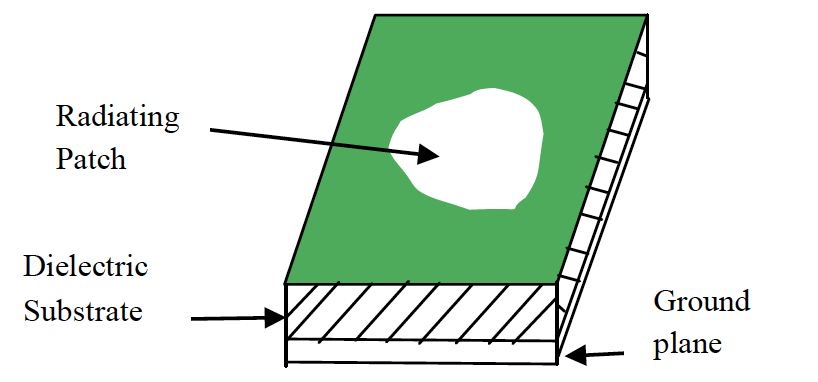
\includegraphics[width=\textwidth/2]{../images/patchantenna.png}
  \caption{General design of a microstrip antenna}
  \label{fig:basicpatchantenna}
\end{figure}

The microstrip antenna requires besides the groundplane, dielectric substrate and the radiation patch also a feed line. Several feeding techniques exists of which the most popular are: coaxial probe feeding, microstrip line and apeture coupling. %and Microstrip Patch Antenna
(todo: more refs? gebruik nummer twee van J13 (p2))

A first feeding method is with the usage of a coaxial cable where the outer conductor is attached to the ground plane and the inner conductor to the radiations patch. Modelling is however difficult, escpecially for thic substrates as will be used in this master dissertation.
A second option is the usage of a microstrip line. This type of feeding is much easier to model since the microstrip line can be seen as en extension of the radiating patch.
A disadvantage is the increased \gls{spuriousradiation} which limits bandwith.
A third is proximity coupling which has the largest bandwidth and low \gls{spuriousradiation}. It consist however of two dielectric substrates causing the overall thickness
of the antenna to increase as well as it's fabrication difficulty.
(todo: tekst te weinig, bespreek ook apperture coupled attenna (zelfde paper als de rest))

The increasing usage of the microstrip patch antennae can be explained by it's easy fabrication and lightweightness and therefore knows a widespread application in the millitary, global possitioning systems, telemedicine, WiMax applications and so on.
The authors of \cite{J13_microstripadvantages} also state that some of the disadvantages like lower gain and power handling can be solved with the usage of an array configuration.

The radiating patch is usually made of a thin layer of either gold or copper \cite{J14_antennadesign,J15_antennadesign}
and can be any form. However, shapes besides a circle or rectangle would require large numerical computation \cite{J14_antennadesign}.
A simple rectangular shape will thus be used.
Further is also the dielectric constant of the substrate important which typically varies between 2.2 and 12. Finding a good dielectric depends on how the antenna will used. A lower
dielectric constant with a thick substrate will result in better performance, better efficiency and larger bandwidths  \cite{J15_antennadesign}.
On the other hand, a larger dielectric constant reduce de dimensions of the antenna \cite{J14_antennadesign}
which is also useful when attaching the 
antenna to a limited surface. Glass as a dielectric substrate with a constant of 4.4 will therefore be used.
\chapter{Deployment tool}
\label{chap:deploymenttool}

Schrijf over hoe die exposure nu toegevoegd is aan de tool. 
-Wat deed de tool al? Users en femtocell's uniform verdelen op publiek transport, uabs etc
- dat de exposure pas op het einde wordt berekend nadat het netwerk gemodeleerd is.

Algorithm \ref{alg:getexposure} describes the implementation on how to calculate the exposure of a user towards a single base station as described in formula \ref{eq:singleexposure}.
Several values need to be known for this to work. In the first place, the path loss is calculated.  However, the different path loss values are already calculated during the network initialization phase and can, therefore, be reused on the condition they were saved. By only calculating the path loss once,  the time complexity of the tool decreases drastically. 
Afther this, the gain is calculated by adding the antenna gain to the  current input power of the antenna and by substracting the feeder loss as already stated in equation \ref{eq:eirp}.
In the last place, equation \ref{eq:singleexposure} is used and the exposure is returned.

\begin{algorithm}
	\caption{getExposure} 
	\label{alg:getexposure}
     \hspace*{\algorithmicindent} \textbf{Input} user, basestation\\
     \hspace*{\algorithmicindent} \textbf{Output} exposure of a user towards a single basestation
	\begin{algorithmic}[1]
        \State $PL \gets$ path loss between user and basestation
        \State $gain \gets$ getBSantennagain + basestation.getInputPower - getBSFeederLoss
		\State $exposure \gets 10^{\frac{EIRP - 43.15 + 20*\log(f)- PL}{20}}$\\
    \Return $exposure$ 
	\end{algorithmic} 
\end{algorithm}

To combine all exposures for a specific user, equation \ref{eq:totalexposure} is translated into algortim \ref{alg:gettotalexposure}.
Finaly, this needs to be repeaded for every users. Algorithm \ref{alg:main} is used to iterate over each user and each simulation and saves the computed value
into the appropriate attribute.

\begin{algorithm}
	\caption{getTotalExposure} 
	\label{alg:gettotalexposure}
     \hspace*{\algorithmicindent} \textbf{Input} user, basestations[]\\
     \hspace*{\algorithmicindent} \textbf{Output} combined exposures from each basestation for a given user
	\begin{algorithmic}[1]
        \State $E_{tot}\gets 0.0$
		\ForAll {basestation  in  basestations}
            \State $E \gets$ getExposure(user, basestation)
            \State $E_{tot}\gets E_{tot} + E^2$	
		\EndFor
        \State $E_{tot}\gets sqrt(E_{tot})$\\
    \Return $E_{tot}$ 
	\end{algorithmic} 
\end{algorithm}

\begin{algorithm}
	\caption{Calculate and save the total exposure for each user in each simulation} 
	\label{alg:main}
     \hspace*{\algorithmicindent} \textbf{Input} users[][], basestations[][]\\
     \hspace*{\algorithmicindent} \textbf{Output} /
	\begin{algorithmic}[1]
		\For {$simulation=1,2,\ldots basestations$}
			\ForAll {user  in  users[simulation]}
				\State $user.exposure \gets  getTotalExposure(user,basestations[simulation])$
			\EndFor
		\EndFor
	\end{algorithmic} 
\end{algorithm}

To provide a summary of how the network is performing on electromagnetic exposure, a weighted average is calculated. This is implemented in algorithm \ref{alg:getglobaluserexposure} which
takes all users for a specified simulation and two weighting factors $w_1$ and $w_2$. They respectively correspond to the 50th percentile and 95th of the ordered users' exposure. The two weights get equal importance of 0.5. This is because also higher values should be taken into account and not compensated with very low values. The formula will only use electric field strengths where users are active as opposed to \cite{J1} where the area is divided into grids and the exposure is calculated for every gridpoint. The reasoning behind this is that the goal of this master dissertation is to calculate the average exposure of the user and not of the entire area.

The formula first calculates the index where the mean value and the 95th percentile should be located. Afterwards, the exposure is calculated using interpolation if necessary.

\begin{algorithm}
	\caption{globalUserExpsoure} 
	\label{alg:getglobaluserexposure}
     \hspace*{\algorithmicindent} \textbf{Input} users[], $w_1$, $w_2$\\
     \hspace*{\algorithmicindent} \textbf{Output} Weighted average of the median  and the $95th$ percentile electric field strenght
	\begin{algorithmic}[1]
		\State Sort users by $E_{tot}$
		
 		\Comment{E50}
		\State $meanIndex \gets \frac{users.length}{2}$
		\If{users.length \% 2 == 0}
			\State $E_{50} \gets users[meanIndex].exposure$ 
		\Else
			\State $E_{50} \gets \frac{(users[ \left \lceil{meanIndex}\right \rceil ].exposure) + (users[ \left \lfloor{meanIndex}\right \rfloor ].exposure)}{2}$ 
		\EndIf

		\Comment{E95 with interpolation}
		\State $ X \gets users.length * 0.95$ 
		\State $ X_1 \gets \left \lfloor{x}\right \rfloor $ 
		\State $ X_2 \gets \left \lceil{x}\right \rceil $ 
		\State $ Y_1 \gets users[X_1].exposure$ 
		\State $ Y_2 \gets users[X_2].exposure$ 
		\State $E_{95} \gets  Y_1 + \left(\frac{(X - X_1)}{(X_2 - X_1)}* (Y_2 - Y_1)\right)$\\
		\Return $\frac{(w_1* E_{50})+ (w_2 * E_{95})}{w_1 + w_2}$
	\end{algorithmic} 
\end{algorithm}
\chapter{Implementation}
\label{chap:implementation}

\section{Implementation of downlink exposure}
\label{sec:downlinkimplementation}

Schrijf over hoe die exposure nu toegevoegd is aan de tool. 
-Wat deed de tool al? Users en femtocell's uniform verdelen op publiek transport, uabs etc
- dat de exposure pas op het einde wordt berekend nadat het netwerk gemodeleerd is.

Algorithm \ref{alg:getexposure} describes the implementation on how to calculate the exposure of a user towards a single base station as described in formula \ref{eq:singleexposure}.
Several values need to be known for this to work. In the first place, the path loss is calculated.  However, the different path loss values are already calculated during the network initialization phase and can, therefore, be reused on the condition they were saved. By only calculating the path loss once,  the time complexity of the tool decreases drastically. 
Afther this, the gain is calculated by adding the antenna gain to the  current input power of the antenna and by substracting the feeder loss as already stated in equation \ref{eq:eirp}.
In the last place, equation \ref{eq:singleexposure} is used and the exposure is returned.

\begin{algorithm}
	\caption{getExposure} 
	\label{alg:getexposure}
     \hspace*{\algorithmicindent} \textbf{Input} user, basestation\\
     \hspace*{\algorithmicindent} \textbf{Output} exposure of a user towards a single basestation
	\begin{algorithmic}[1]
        \State $PL \gets$ path loss between user and basestation
        \State $gain \gets$ getBSantennagain + basestation.getInputPower - getBSFeederLoss
		\State $exposure \gets 10^{\frac{EIRP - 43.15 + 20*\log(f)- PL}{20}}$ \\
    \Return $exposure$ 
	\end{algorithmic} 
\end{algorithm}

To combine all exposures for a specific user, equation \ref{eq:totalexposure} is translated into algortim \ref{alg:gettotalexposure}.
Finaly, this needs to be repeaded for every users. Algorithm \ref{alg:main} is used to iterate over each user and each simulation and saves the computed value
into the appropriate attribute.

\begin{algorithm}
	\caption{getTotalExposure} 
	\label{alg:gettotalexposure}
     \hspace*{\algorithmicindent} \textbf{Input} user, basestations[]\\
     \hspace*{\algorithmicindent} \textbf{Output} combined exposures from each basestation for a given user
	\begin{algorithmic}[1]
        \State $E_{tot}\gets 0.0$
		\ForAll {basestation  in  basestations}
            \State $E \gets$ getExposure(user, basestation)
            \State $E_{tot}\gets E_{tot} + E^2$	
		\EndFor
        \State $E_{tot}\gets sqrt(E_{tot})$\\
    \Return $E_{tot}$ 
	\end{algorithmic} 
\end{algorithm}

\begin{algorithm}
	\caption{Calculate and save the total exposure for each user in each simulation} 
	\label{alg:main}
     \hspace*{\algorithmicindent} \textbf{Input} users[][], basestations[][]\\
     \hspace*{\algorithmicindent} \textbf{Output} /
	\begin{algorithmic}[1]
		\For {$simulation=1,2,\ldots basestations$}
			\ForAll {user  in  users[simulation]}
				\State $user.exposure \gets  getTotalExposure(user,basestations[simulation])$
			\EndFor
		\EndFor
	\end{algorithmic} 
\end{algorithm}

To provide a summary of how the network is performing on electromagnetic exposure, a weighted average is calculated. This is implemented in algorithm \ref{alg:getglobaluserexposure} which
takes all users for a specified simulation and two weighting factors $w_1$ and $w_2$. They respectively correspond to the 50th percentile and 95th of the ordered users' exposure. The two weights get equal importance of 0.5. This is because also higher values should be taken into account and not compensated with very low values. The formula will only use electric field strengths where users are active as opposed to \cite{J1} where the area is divided into grids and the exposure is calculated for every gridpoint. The reasoning behind this is that the goal of this master dissertation is to calculate the average exposure of the user and not of the entire area.

The formula first calculates the index where the mean value and the 95th percentile should be located. Afterwards, the exposure is calculated using interpolation if necessary.

\begin{algorithm}
	\caption{globalUserExpsoure} 
	\label{alg:getglobaluserexposure}
     \hspace*{\algorithmicindent} \textbf{Input} users[], $w_1$, $w_2$\\
     \hspace*{\algorithmicindent} \textbf{Output} Weighted average of the median  and the $95th$ percentile electric field strenght
	\begin{algorithmic}[1]
		\State Sort users by $E_{tot}$
		
 		\Comment{E50}
		\State $meanIndex \gets \frac{users.length}{2}$
		\If{users.length \% 2 == 0}
			\State $E_{50} \gets users[meanIndex].exposure$ 
		\Else
			\State $E_{50} \gets \frac{(users[ \left \lceil{meanIndex}\right \rceil ].exposure) + (users[ \left \lfloor{meanIndex}\right \rfloor ].exposure)}{2}$ 
		\EndIf

		\Comment{E95 with interpolation}
		\State $ X \gets users.length * 0.95$ 
		\State $ X_1 \gets \left \lfloor{x}\right \rfloor $ 
		\State $ X_2 \gets \left \lceil{x}\right \rceil $ 
		\State $ Y_1 \gets users[X_1].exposure$ 
		\State $ Y_2 \gets users[X_2].exposure$ 
		\State $E_{95} \gets  Y_1 + \left(\frac{(X - X_1)}{(X_2 - X_1)}* (Y_2 - Y_1)\right)$\\
		\Return $\frac{(w_1* E_{50})+ (w_2 * E_{95})}{w_1 + w_2}$
	\end{algorithmic} 
\end{algorithm}

%%%%%%%%%%%%%%%%%%%%%%%%% SECTIOIN %%%%%%%%%%%%%%%%%%%%%%%%
\section{Implementation of uplink exposure}
\label{sec:uplinkexposure}

Analogously to the \ref{sec:downlinkimplementation}, the uplink calculator will determine the uplink exposure and save in the appropriate user object. The calculator starts with iterating over each user in each simulation and calls the getSar() function.

\ref{eq:sar10g} is implemented in \ref{algo:getsar}. The function requires a user as input for which the uplink exposure should be calculated and two constant values which should be declared once. The maximal allowed $SAR_{10g}$ as discussed in \ref{sec:sar} and maximal permitted transmission power of 23 dbm.

Also, the actual transmitting power of the \gls{UE} needs to be calculated using the getActualTransmitPower function. 

Both $Tx_{watt}$ and $TX^{max}_{watt}$ are converted to watt. This is because the decibel variant can range from -57 dBm to 23 dBm \cite{J10_RDPgit}. Converting to Watt results in a solely positive fraction. 

After having multiplied with the maximum allowable \gls{SAR}, the actual uplink exposure is returned.

\begin{algorithm}
	\caption{getSar} 
	\label{alg:getsar}
     \hspace*{\algorithmicindent} \textbf{Input} user \\
     \hspace*{\algorithmicindent} \textbf{Output} $SAR_{10g}$
	\begin{algorithmic}[1]
		\State  const $SAR^{max} \gets 0.67$
		\State  const $TX^{max}_{watt} \gets dBm2W(23)$
		\vspace{4 mm}
		\State $Tx_{watt} \gets dBm2W(getActualTransmitPower(user)) $		
		\State $ SAR_{10g} \gets \frac{Tx_{watt}}{TX^{max}_{watt}} * SAR^{max}$ \\
		\Return $ SAR_{10g}$
	\end{algorithmic} 
\end{algorithm}


The implementation for getActualTransmitPower is described in \ref{alg:getActualTransmitPower}. This function requires a user as a parameter and will calculate the real used power for transmission in dBm.
Once again, a global constant value is defined describing the maximum allowable transmitting power $Tx^{max}_{dBm}$ expressed in dBm. The predicted transmitting power is achieved by subtracting the path loss between the user and the affective femtocell with the receiver sensitivity of the femtocell. However, this value can't be higher then  $Tx^{max}_{dBm}$ , if this is the case the maximum allowable transmitting power is returned instead.

\begin{algorithm}
	\caption{getActualTransmitPower} 
	\label{alg:getActualTransmitPowergit}
     \hspace*{\algorithmicindent} \textbf{Input} user \\
     \hspace*{\algorithmicindent} \textbf{Output} The actual used power for transmition in dBm.
	\begin{algorithmic}[1]
		\State const $Tx^{max}_{dBm} \gets 23$
		\vspace{4 mm}
		\State $ Tx_{dBm} \gets user.getPathLoss() - technology.getFemtocellReceiverSensitivity(user.getRxSNR)$ \\
		\Return $min(Tx_{dBm}, Tx^{max}_{dBm})$ 
	\end{algorithmic} 
\end{algorithm}


%\begin{algorithm}
%	\caption{getFemtocellReceiverSensitivity} 
%	\label{alg:getFemtocellReceiverSensitivity}
%     \hspace*{\algorithmicindent} \textbf{Input} user \\
%     \hspace*{\algorithmicindent} \textbf{Output} The receiver sensitivity of the femtocell in dBm
%	\begin{algorithmic}[1]
%		\State $SNR \gets user.getRxSNR$
%		\State $gain \gets technology.getMSantennagain$
%		\State $implementationLoss \gets technology.getImplementationLoss$
%		\State $interferenceMargin \gets technology.getCellInterferenceMargin$
%		\State $noiseFigure \gets technology.getNoiseFigure$
%		\State $thermalNoise \gets -108.1$	\\
%		\Return  $thermalNoise + SNR - gain + implementationLoss + noiseFigure + interferenceMargin$
%	\end{algorithmic} 
%\end{algorithm}


\chapter{Scenarios}
\label{chap:scenarios}


\chapter{Conclusions}
\label{chap:Conclusions}
\bibliographystyle{ieeetr}
\bibliography{referenties}

\chapter{pseudocode}
\label{chap:pseudocode}

\section{Implementation of downlink exposure}
\label{sec:downlinkimplementation}

Schrijf over hoe die exposure nu toegevoegd is aan de tool. 
-Wat deed de tool al? Users en femtocell's uniform verdelen op publiek transport, uabs etc
- dat de exposure pas op het einde wordt berekend nadat het netwerk gemodeleerd is.

Algorithm \ref{alg:getexposure} describes the implementation on how to calculate the exposure of a user towards a single base station as described in formula \ref{eq:singleexposure}.
Several values need to be known for this to work. In the first place, the path loss is calculated.  However, the different path loss values are already calculated during the network initialization phase and can, therefore, be reused on the condition they were saved. By only calculating the path loss once,  the time complexity of the tool decreases drastically. 
Afther this, the gain is calculated by adding the antenna gain to the  current input power of the antenna and by substracting the feeder loss as already stated in equation \ref{eq:eirp}.
In the last place, equation \ref{eq:singleexposure} is used and the exposure is returned.

\begin{algorithm}
	\caption{getExposure} 
	\label{alg:getexposure}
     \hspace*{\algorithmicindent} \textbf{Input} user, basestation\\
     \hspace*{\algorithmicindent} \textbf{Output} exposure of a user towards a single basestation
	\begin{algorithmic}[1]
        \State $PL \gets$ path loss between user and basestation
        \State $gain \gets$ getBSantennagain + basestation.getInputPower - getBSFeederLoss
		\State $exposure \gets 10^{\frac{EIRP - 43.15 + 20*\log(f)- PL}{20}}$ \\
    \Return $exposure$ 
	\end{algorithmic} 
\end{algorithm}

To combine all exposures for a specific user, equation \ref{eq:totalexposure} is translated into algortim \ref{alg:gettotalexposure}.
Finaly, this needs to be repeaded for every users. Algorithm \ref{alg:main} is used to iterate over each user and each simulation and saves the computed value
into the appropriate attribute.

\begin{algorithm}
	\caption{getTotalExposure} 
	\label{alg:gettotalexposure}
     \hspace*{\algorithmicindent} \textbf{Input} user, basestations[]\\
     \hspace*{\algorithmicindent} \textbf{Output} combined exposures from each basestation for a given user
	\begin{algorithmic}[1]
        \State $E_{tot}\gets 0.0$
		\ForAll {basestation  in  basestations}
            \State $E \gets$ getExposure(user, basestation)
            \State $E_{tot}\gets E_{tot} + E^2$	
		\EndFor
        \State $E_{tot}\gets sqrt(E_{tot})$\\
    \Return $E_{tot}$ 
	\end{algorithmic} 
\end{algorithm}

\begin{algorithm}
	\caption{Calculate and save the total exposure for each user in each simulation} 
	\label{alg:main}
     \hspace*{\algorithmicindent} \textbf{Input} users[][], basestations[][]\\
     \hspace*{\algorithmicindent} \textbf{Output} /
	\begin{algorithmic}[1]
		\For {$simulation=1,2,\ldots basestations$}
			\ForAll {user  in  users[simulation]}
				\State $user.exposure \gets  getTotalExposure(user,basestations[simulation])$
			\EndFor
		\EndFor
	\end{algorithmic} 
\end{algorithm}

To provide a summary of how the network is performing on electromagnetic exposure, a weighted average is calculated. This is implemented in algorithm \ref{alg:getglobaluserexposure} which
takes all users for a specified simulation and two weighting factors $w_1$ and $w_2$. They respectively correspond to the 50th percentile and 95th of the ordered users' exposure. The two weights get equal importance of 0.5. This is because also higher values should be taken into account and not compensated with very low values. The formula will only use electric field strengths where users are active as opposed to \cite{J1} where the area is divided into grids and the exposure is calculated for every gridpoint. The reasoning behind this is that the goal of this master dissertation is to calculate the average exposure of the user and not of the entire area.

The formula first calculates the index where the mean value and the 95th percentile should be located. Afterwards, the exposure is calculated using interpolation if necessary.

\begin{algorithm}
	\caption{globalUserExpsoure} 
	\label{alg:getglobaluserexposure}
     \hspace*{\algorithmicindent} \textbf{Input} users[], $w_1$, $w_2$\\
     \hspace*{\algorithmicindent} \textbf{Output} Weighted average of the median  and the $95th$ percentile electric field strenght
	\begin{algorithmic}[1]
		\State Sort users by $E_{tot}$
		
 		\Comment{E50}
		\State $meanIndex \gets \frac{users.length}{2}$
		\If{users.length \% 2 == 0}
			\State $E_{50} \gets users[meanIndex].exposure$ 
		\Else
			\State $E_{50} \gets \frac{(users[ \left \lceil{meanIndex}\right \rceil ].exposure) + (users[ \left \lfloor{meanIndex}\right \rfloor ].exposure)}{2}$ 
		\EndIf

		\Comment{E95 with interpolation}
		\State $ X \gets users.length * 0.95$ 
		\State $ X_1 \gets \left \lfloor{x}\right \rfloor $ 
		\State $ X_2 \gets \left \lceil{x}\right \rceil $ 
		\State $ Y_1 \gets users[X_1].exposure$ 
		\State $ Y_2 \gets users[X_2].exposure$ 
		\State $E_{95} \gets  Y_1 + \left(\frac{(X - X_1)}{(X_2 - X_1)}* (Y_2 - Y_1)\right)$\\
		\Return $\frac{(w_1* E_{50})+ (w_2 * E_{95})}{w_1 + w_2}$
	\end{algorithmic} 
\end{algorithm}

%%%%%%%%%%%%%%%%%%%%%%%%% SECTIOIN %%%%%%%%%%%%%%%%%%%%%%%%
\section{Implementation of uplink exposure}
\label{sec:uplinkexposure}

Analogously to the \ref{sec:downlinkimplementation}, the uplink calculator will determine the uplink exposure and save in the appropriate user object. The calculator starts with iterating over each user in each simulation and calls the getSar() function.

\ref{eq:sar10g} is implemented in \ref{algo:getsar}. The function requires a user as input for which the uplink exposure should be calculated and two constant values which should be declared once. The maximal allowed $SAR_{10g}$ as discussed in \ref{sec:sar} and maximal permitted transmission power of 23 dbm.

Also, the actual transmitting power of the \gls{UE} needs to be calculated using the getActualTransmitPower function. 

Both $Tx_{watt}$ and $TX^{max}_{watt}$ are converted to watt. This is because the decibel variant can range from -57 dBm to 23 dBm \cite{J10_RDPgit}. Converting to Watt results in a solely positive fraction. 

After having multiplied with the maximum allowable \gls{SAR}, the actual uplink exposure is returned.

\begin{algorithm}
	\caption{getSar} 
	\label{alg:getsar}
     \hspace*{\algorithmicindent} \textbf{Input} user \\
     \hspace*{\algorithmicindent} \textbf{Output} $SAR_{10g}$
	\begin{algorithmic}[1]
		\State  const $SAR^{max} \gets 0.67$
		\State  const $TX^{max}_{watt} \gets dBm2W(23)$
		\vspace{4 mm}
		\State $Tx_{watt} \gets dBm2W(getActualTransmitPower(user)) $		
		\State $ SAR_{10g} \gets \frac{Tx_{watt}}{TX^{max}_{watt}} * SAR^{max}$ \\
		\Return $ SAR_{10g}$
	\end{algorithmic} 
\end{algorithm}


The implementation for getActualTransmitPower is described in \ref{alg:getActualTransmitPower}. This function requires a user as a parameter and will calculate the real used power for transmission in dBm.
Once again, a global constant value is defined describing the maximum allowable transmitting power $Tx^{max}_{dBm}$ expressed in dBm. The predicted transmitting power is achieved by subtracting the path loss between the user and the affective femtocell with the receiver sensitivity of the femtocell. However, this value can't be higher then  $Tx^{max}_{dBm}$ , if this is the case the maximum allowable transmitting power is returned instead.

\begin{algorithm}
	\caption{getActualTransmitPower} 
	\label{alg:getActualTransmitPowergit}
     \hspace*{\algorithmicindent} \textbf{Input} user \\
     \hspace*{\algorithmicindent} \textbf{Output} The actual used power for transmition in dBm.
	\begin{algorithmic}[1]
		\State const $Tx^{max}_{dBm} \gets 23$
		\vspace{4 mm}
		\State $ Tx_{dBm} \gets user.getPathLoss() - technology.getFemtocellReceiverSensitivity(user.getRxSNR)$ \\
		\Return $min(Tx_{dBm}, Tx^{max}_{dBm})$ 
	\end{algorithmic} 
\end{algorithm}


%\begin{algorithm}
%	\caption{getFemtocellReceiverSensitivity} 
%	\label{alg:getFemtocellReceiverSensitivity}
%     \hspace*{\algorithmicindent} \textbf{Input} user \\
%     \hspace*{\algorithmicindent} \textbf{Output} The receiver sensitivity of the femtocell in dBm
%	\begin{algorithmic}[1]
%		\State $SNR \gets user.getRxSNR$
%		\State $gain \gets technology.getMSantennagain$
%		\State $implementationLoss \gets technology.getImplementationLoss$
%		\State $interferenceMargin \gets technology.getCellInterferenceMargin$
%		\State $noiseFigure \gets technology.getNoiseFigure$
%		\State $thermalNoise \gets -108.1$	\\
%		\Return  $thermalNoise + SNR - gain + implementationLoss + noiseFigure + interferenceMargin$
%	\end{algorithmic} 
%\end{algorithm}



\end{document}
